\subsection*{Диграмма последовательностей}

% UML диаграмма последовательности (Sequence diagram) - это диаграмма, которая отображает взаимодействие между объектами или компонентами в системе
% в виде последовательности сообщений, которые передаются между ними.

% Диаграмма последовательностей спроектирована в draw.io \cite{drawio} и изображена на рис.~\ref{fig:UML_sequence_diagram}.

% UML диаграмма последовательности позволяет представить взаимодействие между объектами в форме временной последовательности,
% показывая, как каждый объект взаимодействует с другими и когда это происходит. Объекты изображаются в виде вертикальных линий (жизненных линий),
% а сообщения между объектами отображаются в виде стрелок, которые указывают направление передачи информации.

UML (Unified Modeling Language) диаграмма последовательностей (англ. sequence diagram) отображает
взаимодействие объектов или компонентов в виде вертикальных линий, известных как <<жизненные линии>>.
По мере выполнения определенных действий или вызова методов,
сообщения и события передаются между участниками системы,
что отображается в виде стрелок, соединяющих соответствующие жизненные линии.
Это позволяет легко проследить порядок выполнения операций и взаимодействие между различными элементами системы.

На рисунке~\ref{fig:UML_sequence_diagram} представлена диаграмма последовательностей,
демонстрирующая взаимодействие между мобильным приложением, серверной частью и базой данных.

\begin{figure}[!htb]
    \centering

    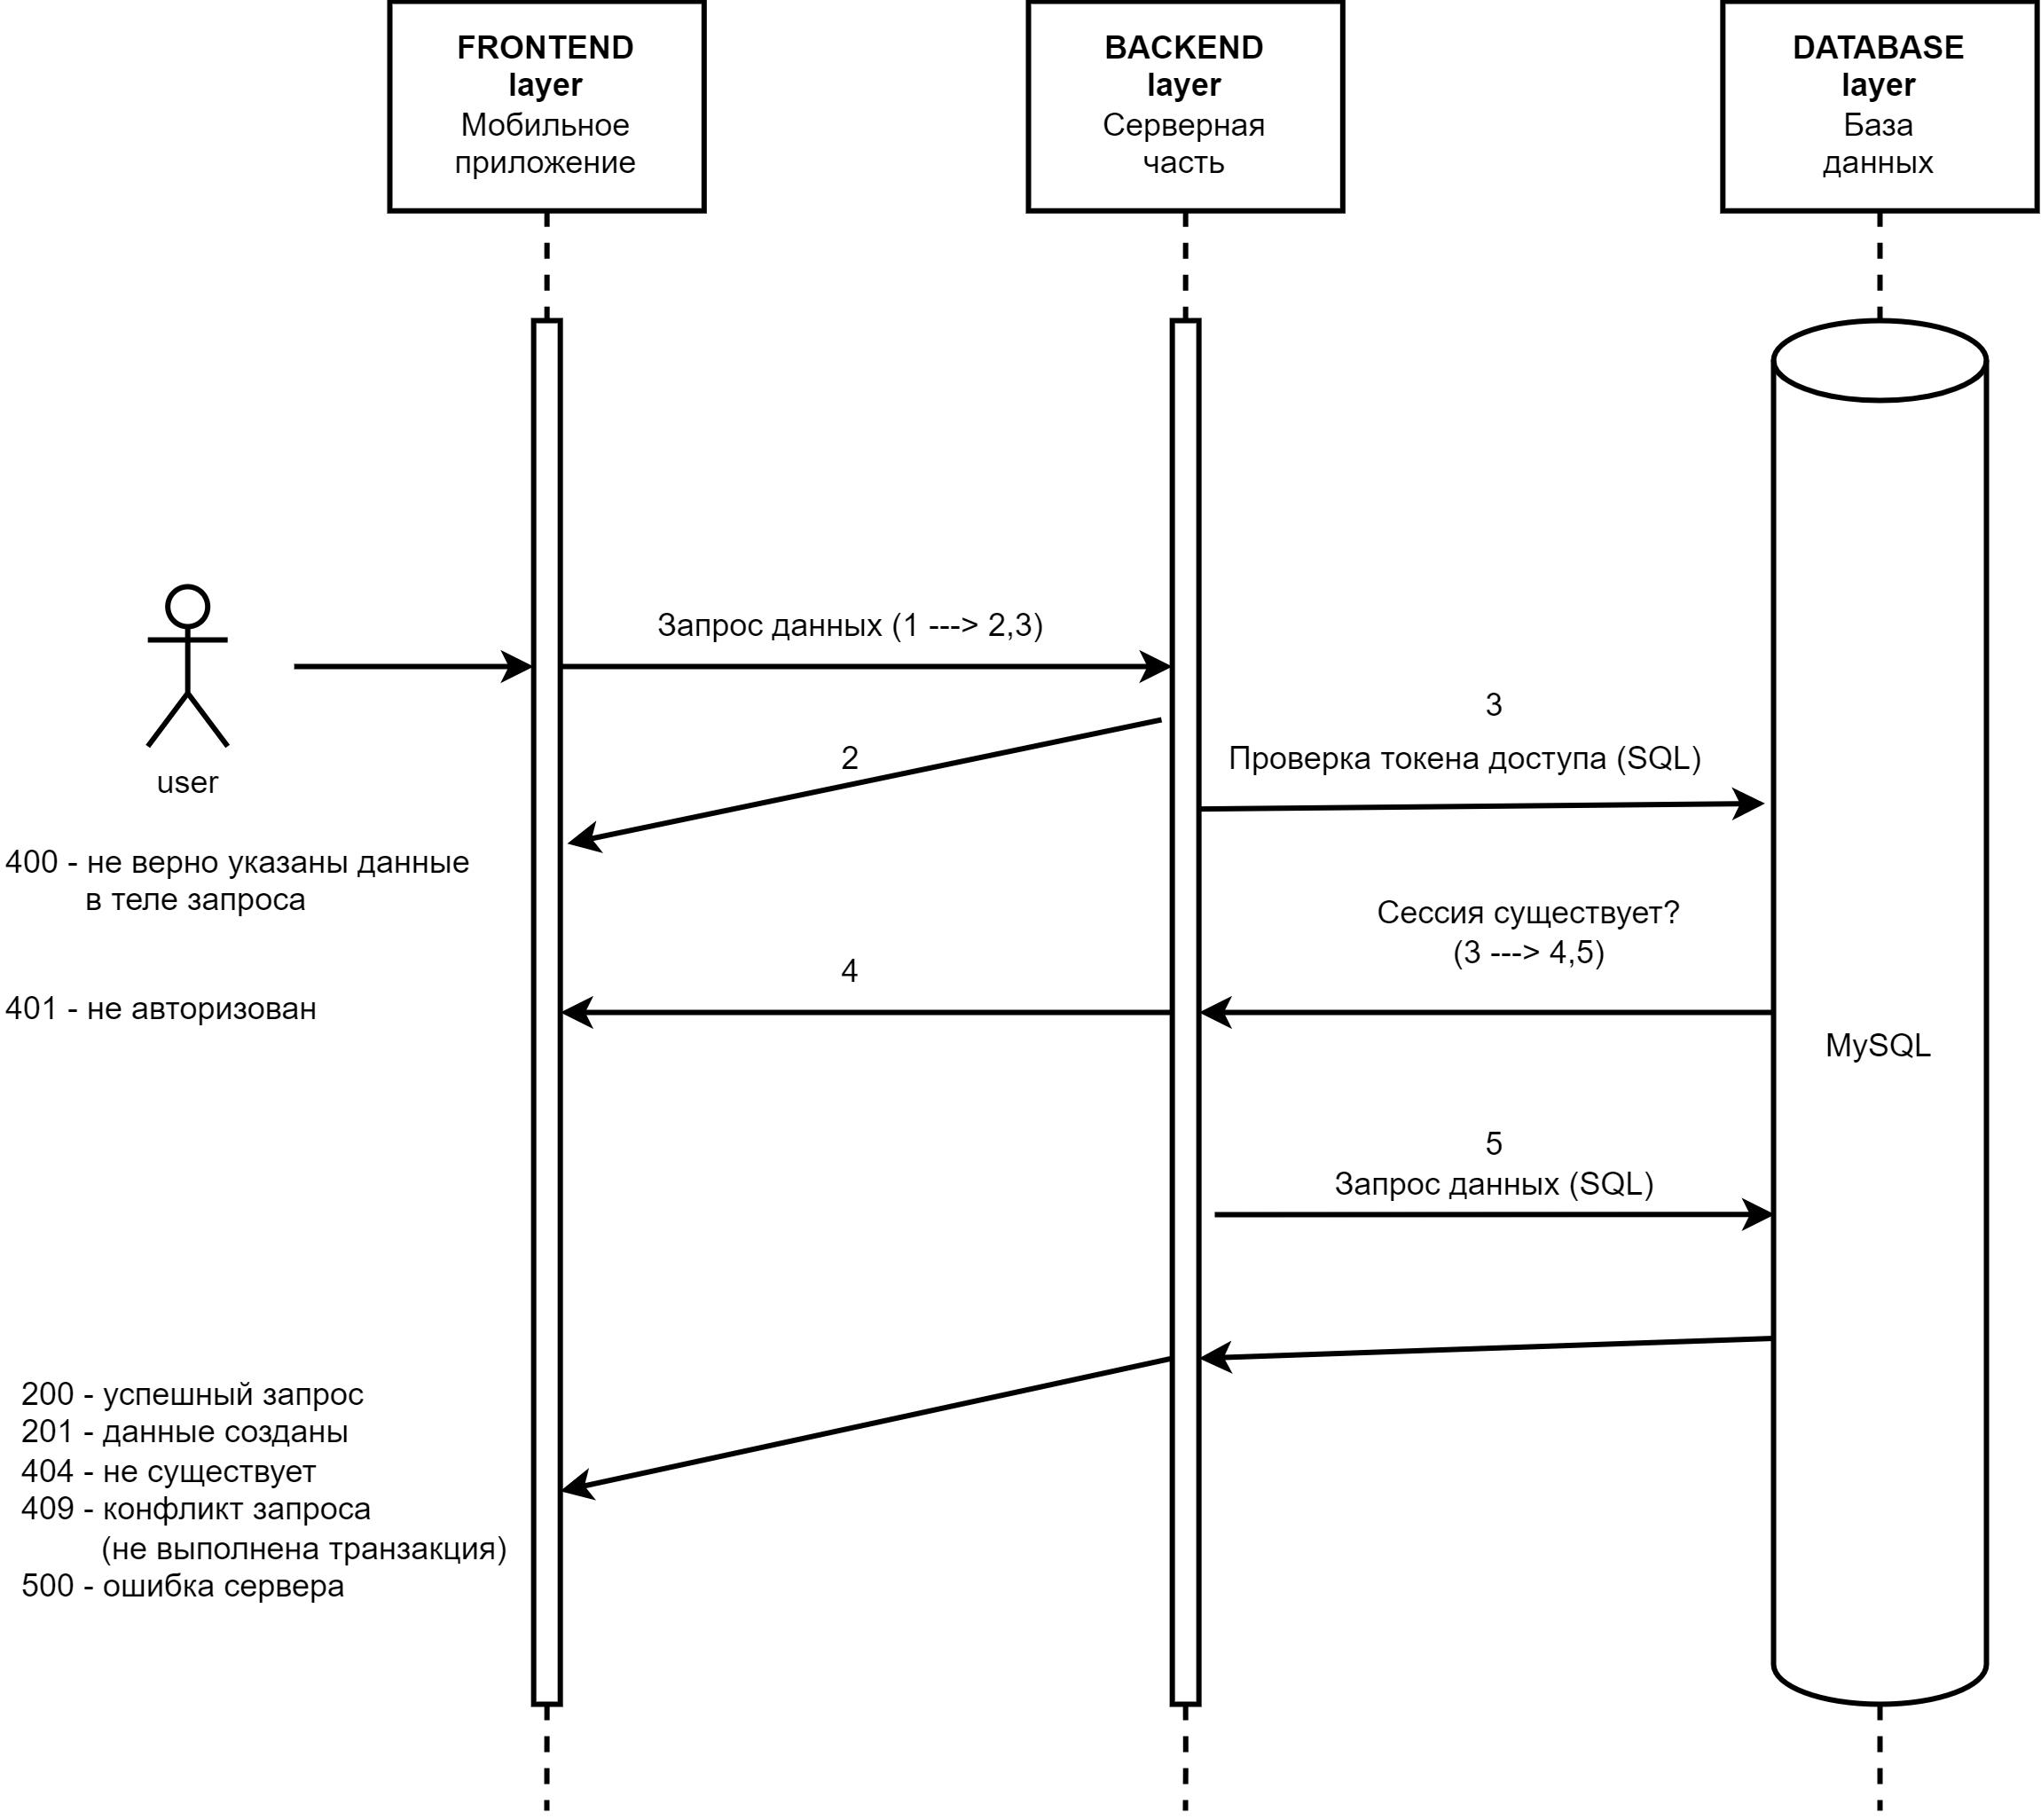
\includegraphics[width=14cm]
    {images/UML/sequence/sequence.png}

    \caption{Диаграмма последовательностей}

    \label{fig:UML_sequence_diagram}
\end{figure}
